\documentclass[12pt,a4paper]{article}
\usepackage[utf8]{inputenc}
\usepackage[margin=1in]{geometry}
\usepackage{amsmath,amssymb,amsfonts}
\usepackage{graphicx}
\usepackage{booktabs}
\usepackage{tabularx}
\usepackage{hyperref}
\usepackage{cite}
\usepackage{listings}
\usepackage{xcolor}
\usepackage{setspace}
\usepackage{titlesec}
\usepackage{caption}
\usepackage{subcaption}
\usepackage{tikz}
\usetikzlibrary{shapes.geometric, arrows, positioning}

\hypersetup{
    colorlinks=true,
    linkcolor=black,
    citecolor=blue!70!black,
    filecolor=black,
    urlcolor=blue!70!black
}

\onehalfspacing

% Code Listing Styling
\lstset{
    basicstyle=\ttfamily\footnotesize,
    breaklines=true,
    captionpos=b,
    frame=single,
    showstringspaces=false,
    commentstyle=\color{gray},
    keywordstyle=\color{blue},
    stringstyle=\color{teal}
}

\begin{document}

% ==========================================
% TITLE PAGE (Matching Aeropendulum Report Layout)
% ==========================================
\begin{titlepage}
    \centering
    \vspace*{1.5cm}
    
    {\Large \bfseries DESIGN, MODELLING AND EVALUATION OF A \\ PHYSICS-INFORMED NEURAL NETWORK FOR \\ EV BATTERY THERMAL DIGITAL TWIN GENERALIZATION \par}
    
    \vspace{1.5cm}
    \rule{\linewidth}{0.5pt}
    \vspace{2.0cm}
    
    {\large Under the Guidance of \par}
    \vspace{0.3cm}
    {\large \bfseries Prof. Rammohan A \par}
    
    \vspace{2.0cm}
    
    {\large Submitted by \par}
    \vspace{0.3cm}
    {\large \bfseries Abimanyu Jayaganesh \par}
    {\large 23BCE2070 \par}
    
    \vfill
    
    {\large \bfseries Automotive Research Centre \par}
    {\large \bfseries Vellore Institute of Technology \par}
    
    \vspace{1.0cm}
    {\large May - July 2026 \par}
\end{titlepage}

% ==========================================
% PRELIMINARY PAGES (Roman Numbering)
% ==========================================
\pagenumbering{roman}
\setcounter{page}{1}

\section*{Abstract}
This report documents an engineering research project in which a Physics-Informed Neural Network (PINN) digital twin framework was designed, modelled, and evaluated for real-time thermal state estimation in lithium-ion battery cells used in electric vehicles (EVs). The battery thermal digital twin is a dynamic mechatronic software plant that operates in parallel with physical battery packs to predict thermal dynamics under dynamic load cycles. The project covered a complete machine learning workflow: selection of lumped electro-thermal physical parameters, formulation of ordinary differential equation (ODE) physics loss constraints, design of a Multi-Layer Perceptron (MLP) architecture, implementation of input noise injection to mitigate exposure bias, and multi-step autoregressive rollout evaluation across unseen test drive cycles (WLTP2). Evaluated on a large-scale dataset comprising 522 simulated trajectories containing approximately 78 million time steps across multiple drive cycles, ambient temperatures ($0^\circ\text{C}$ to $50^\circ\text{C}$), and cell mass scales, the resulting PINN pipeline reduced the maximum rollout error on an unseen test drive cycle from $0.2474^\circ\text{C}$ in the baseline MLP to $0.0851^\circ\text{C}$, achieving an autoregressive rollout Mean Absolute Error (MAE) of $0.0117^\circ\text{C}$. The trainable convective heat transfer parameter ($hA$) converged via softplus parameterization to an effective value of $36.49~\text{W/K}$, consistent with the single-node thermal model and cell surface cooling dynamics. This report presents the theoretical background, governing mathematical model, software architecture, training methodology, execution benchmarking, and experimental observations gathered over the course of the project.

\newpage

\tableofcontents
\newpage

\listoffigures
\listoftables
\newpage

% ==========================================
% MAIN BODY (Arabic Numbering)
% ==========================================
\pagenumbering{arabic}
\setcounter{page}{1}

\section{Introduction}
The global transition to electric vehicles (EVs) places stringent operational demands on battery management systems (BMS) to ensure safety, maximize performance, and prolong pack service life. Lithium-ion batteries generate substantial internal heat during charge and discharge transients due to internal ohmic resistance and electrochemical reactions. If unmanaged, excessive heat buildup leads to localized thermal hotspots, accelerated capacity fade, and severe thermal runaway hazards. Real-time temperature monitoring at both the cell and pack levels is therefore a critical safety-critical function of modern EV BMS architectures.

Dynamic thermal models serve as the foundation of battery thermal digital twins, running concurrently with physical energy storage systems to predict internal temperature evolution, estimate cooling requirements, and adjust real-time charging limits. Traditionally, high-fidelity thermal modeling has relied on computational fluid dynamics (CFD) or multi-dimensional finite element methods (FEM). While accurate, these methods are computationally heavy and unsuitable for real-time edge execution on vehicle microcontrollers. Consequently, simplified lumped-parameter thermal networks or equivalent circuit models (ECMs) are typically deployed. However, simplified models require extensive manual calibration and struggle to capture rapid transient dynamics under dynamic automotive load profiles.

Recently, data-driven machine learning (ML) models such as Multi-Layer Perceptrons (MLPs) have emerged as rapid surrogates. Despite their speed, purely data-driven models suffer from two critical limitations:
\begin{enumerate}
    \item \textbf{Physical Inconsistency:} Unconstrained neural networks may produce outputs violating thermodynamic laws (e.g., cell temperature dropping despite high current draws and high ambient temperatures) when operating outside training distributions.
    \item \textbf{Exposure Bias and Rollout Drift:} During standard training, models are optimized using single-step-ahead objectives ($T_{t+1}$ given ground-truth $T_t$). In deployment, the digital twin operates recursively, feeding prior predicted temperatures back as inputs. Small single-step errors compound over thousands of evaluation steps, causing accumulating trajectory error. In high-frequency sampling regimes ($dt = 0.01$~s), single-step metrics are misleadingly optimistic because predicting zero temperature change ($\Delta T \approx 0$) acts as an identity shortcut.
\end{enumerate}

To address these challenges, this project presents a Physics-Informed Neural Network (PINN) digital twin framework combining lumped-parameter ODE regularization \cite{bernardi1985general, raissi2019physicsinformed, chen2022physics}, softplus-constrained parameter estimation, and input noise injection inspired by scheduled sampling techniques \cite{bengio2015scheduled, ranzato2015sequence} for exposure-bias mitigation.

\section{Mathematical Model}
The dynamic thermal behavior of the battery cell is modeled as a lumped energy-balance thermodynamic system governed by heat generation and convective surface cooling \cite{bernardi1985general, saha2014lumped}.

\subsection{Modelling Assumptions}
The mathematical model relies on the following key engineering assumptions:
\begin{itemize}
    \item \textbf{Lumped Thermal Mass:} The battery cell behaves as a single thermal node with uniform internal temperature distribution.
    \item \textbf{Dominant Heat Sources:} Heat generation ($P_{\text{loss}}$) is produced by internal resistance Joule heating and polarization losses.
    \item \textbf{Convective Cooling:} Surface heat dissipation follows Newton's law of cooling.
    \item \textbf{Isotropic Scaling:} Variations in cell dimensions are represented by a dimensionless mass scale factor ($\text{MassScale}$).
\end{itemize}

\subsection{Determination of Physical Parameters}
The physical parameters governing the battery cell assembly are summarized in Table \ref{tab:physical_params}.

\begin{table}[h]
\centering
\caption{Calculated engineering parameters of the battery cell assembly.}
\label{tab:physical_params}
\begin{tabularx}{\textwidth}{@{}l l X@{}}
\toprule
Parameter & Value & Description / Source \\
\midrule
Cell Structural Mass ($m$) & $1.0\text{ kg}$ & Nominal cell mass \\
Specific Heat Capacity ($C_p$) & $900.0\text{ J/kg/K}$ & Standard Li-ion thermal capacity \\
Thermal Capacity ($m C_p$) & $900.0\text{ J/K}$ & Lumped heat capacity \\
Initial Convective Parameter ($hA_{\text{init}}$) & $0.1\text{ W/K}$ & Softplus parameter initialization \\
Time Step Resolution ($dt$) & $0.01\text{ s}$ & High-frequency Simulink logging \\
\bottomrule
\end{tabularx}
\end{table}

\subsection{Final Nonlinear Model}
Applying the first law of thermodynamics yields the governing differential equation for cell temperature rate of change:
\begin{equation}
m C_p \cdot \text{MassScale} \frac{dT}{dt} = P_{\text{loss}} - hA (T - T_{\text{amb}})
\label{eq:nonlinear_model}
\end{equation}
where $T$ is the cell temperature (K), $P_{\text{loss}}$ is heat generation rate (W), $T_{\text{amb}}$ is ambient temperature (K), and $hA$ is the convective heat transfer coefficient multiplied by surface area (W/K).

Rearranging for the physical rate of temperature change yields:
\begin{equation}
\frac{dT}{dt} = \frac{P_{\text{loss}} - hA(T - T_{\text{amb}})}{m C_p \cdot \text{MassScale}}
\label{eq:rate_of_change}
\end{equation}

\subsection{Physics Loss and Residual Formulation}
The physics loss measures the residual of governing equation (\ref{eq:rate_of_change}) over each training batch. For a predicted temperature delta $\Delta \hat{T}_i^{\text{phys}}$ in physical units ($^\circ\text{C}$), the residual $R_i$ is expressed in physical units (K/s) as:
\begin{equation}
R_i = \frac{\Delta \hat{T}_i^{\text{phys}}}{dt_i} - \frac{P_{\text{loss}, i} - hA (T_i - T_{\text{amb}, i})}{m C_p \cdot \text{MassScale}_i}
\label{eq:residual}
\end{equation}

The physics regularization loss is computed as:
\begin{equation}
\mathcal{L}_{\text{physics}} = \frac{1}{N} \sum_{i=1}^N R_i^2
\label{eq:loss_physics}
\end{equation}

\subsection{Trainable Parameter Parameterization}
To enforce $hA > 0$ and prevent non-physical negative cooling estimates ($hA < 0$) without causing gradient clipping, $hA$ is parameterized via a unconstrained raw parameter $hA_{\text{raw}}$ through a softplus activation:
\begin{equation}
hA = \text{softplus}(hA_{\text{raw}}) = \ln(1 + e^{hA_{\text{raw}}})
\label{eq:softplus}
\end{equation}

\subsection{PID / Data Loss and Objective Function}
The total PINN training objective combines data fidelity with physics regularization:
\begin{equation}
\mathcal{L}_{\text{total}} = \mathcal{L}_{\text{data}} + \lambda_{\text{phys}} \mathcal{L}_{\text{physics}}
\label{eq:loss_total}
\end{equation}
where $\mathcal{L}_{\text{data}} = \frac{1}{N} \sum_{i=1}^N (\Delta T_i - \Delta \hat{T}_i)^2$ and $\lambda_{\text{phys}} = 0.01$.

\subsection{Closed-Loop Autoregressive Rollout}
During digital twin rollout, temperature is updated recursively:
\begin{equation}
\hat{T}_{t+1} = \hat{T}_t + \Delta \hat{T}_t^{\text{phys}}
\label{eq:rollout_step}
\end{equation}

\section{Experimental Setup}
The digital twin pipeline was constructed using standard hardware, software, and simulation dataset components, summarized in Table \ref{tab:materials}.

\begin{table}[h]
\centering
\caption{Principal software, hardware, and dataset environment specifications.}
\label{tab:materials}
\begin{tabularx}{\textwidth}{@{}l p{5.2cm} X@{}}
\toprule
Component & Material / Specification & Function \\
\midrule
GPU Hardware & NVIDIA RTX 4060 Laptop GPU (8 GB VRAM) & Neural network training acceleration \\
CPU Hardware & Intel Core i7 Processor, 16 GB DDR5 RAM & Data preprocessing \& CPU DataLoader \\
Software Stack & PyTorch 2.4, Python 3.10, CUDA 12.9 & Deep learning framework \\
Dataset & 522 Simulink CSV files (78M time steps) & Electro-thermal simulation dataset \\
Training Split & 435 files (FTP75, UDDS, US06, WLTP1) & Model training \& validation \\
Test Split & 87 files (unseen WLTP2 cycle) & Out-of-distribution test evaluation \\
Features & Temperature, Current, Voltage, SOC, PowerLoss, AmbientTemp, MassScale & Feature input vector (7 dimensions) \\
Target & $\Delta T = T_{t+1} - T_t$ & Physical temperature delta ($^\circ\text{C}$) \\
\bottomrule
\end{tabularx}
\end{table}

\section{Design Process}
The digital twin architecture underwent two major design iterations in software.

\subsection{Iteration 1: Single-Step Data-Driven Baseline}
The initial design adopted a pure feedforward MLP trained on one-step-ahead targets ($T_t \to T_{t+1}$). While single-step test MAE was very low ($< 5 \times 10^{-7}{^\circ}\text{C}$), recursive rollout testing revealed trajectory drift (rollout MAE $0.0170^\circ\text{C}$, maximum error $0.2474^\circ\text{C}$). Analysis suggested the network exploited an identity shortcut ($\Delta T \approx 0$), failing to learn true dynamics due to exposure bias.

\subsection{Iteration 2: Noise-Injected PINN Architecture}
To eliminate exposure bias and enforce physical constraints, Iteration 2 introduced:
\begin{itemize}
    \item \textbf{Input Noise Injection:} Adding Gaussian noise ($\sigma = 0.05^\circ\text{C}$) to input temperature during training to perturb state space.
    \item \textbf{Physics Loss Regularization:} Adding governing ODE residual loss ($\lambda_{\text{phys}} = 0.01$).
    \item \textbf{Softplus Parameter Estimation:} Treating $hA$ as a trainable parameter bounded above zero.
\end{itemize}

Figure \ref{fig:pipeline} illustrates the complete end-to-end digital twin execution pipeline.

\begin{figure}[htbp]
\centering
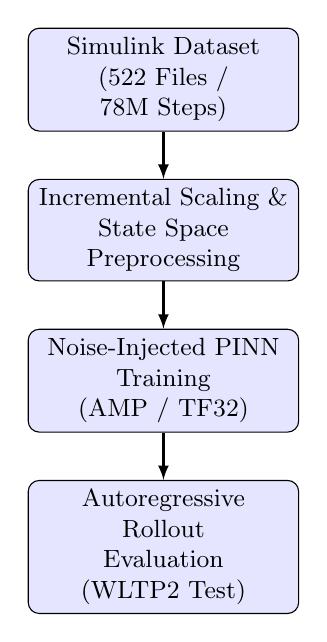
\begin{tikzpicture}[
    auto,
    block/.style={rectangle, draw, fill=blue!10, text width=3.2cm, text centered, rounded corners, minimum height=1.0cm, font=\small},
    line/.style={draw, -latex, thick}
]
    \node [block] (simulink) {Simulink Dataset\\(522 Files / 78M Steps)};
    \node [block, below=0.6cm of simulink] (preprocess) {Incremental Scaling \&\\State Space Preprocessing};
    \node [block, below=0.6cm of preprocess] (train) {Noise-Injected PINN\\Training (AMP / TF32)};
    \node [block, below=0.6cm of train] (eval) {Autoregressive Rollout\\Evaluation (WLTP2 Test)};
    
    \path [line] (simulink) -- (preprocess);
    \path [line] (preprocess) -- (train);
    \path [line] (train) -- (eval);
\end{tikzpicture}
\caption{The battery thermal digital twin pipeline from Simulink data generation to autoregressive rollout evaluation.}
\label{fig:pipeline}
\end{figure}

\section{Network Architecture and Hyperparameters}
The deep neural network architecture and optimization hyperparameters are listed in Table \ref{tab:hyperparams}.

\begin{table}[h]
\centering
\caption{Principal network architecture and optimization hyperparameters.}
\label{tab:hyperparams}
\begin{tabularx}{\textwidth}{@{}l l X@{}}
\toprule
Dimension / Parameter & Approx. Value & Notes \\
\midrule
Input Dimension & 7 features & $[T, I, V, \text{SOC}, P_{\text{loss}}, T_{\text{amb}}, \text{MassScale}]$ \\
Hidden Layers & 3 layers & Layer sizes: 64, 64, 32 \\
Activation Function & ReLU & Non-linear activation \\
Output Dimension & 1 target & Temperature delta ($\Delta T$) \\
Batch Size & 8,192 & Optimized for GPU throughput \\
Optimizer & Adam ($\alpha = 0.001$) & $\beta_1 = 0.9, \beta_2 = 0.999$ \\
Physics Loss Weight ($\lambda_{\text{phys}}$) & $0.01$ & Regularization scaling factor \\
Gaussian Noise ($\sigma$) & $0.05^\circ\text{C}$ & Temperature input noise injection \\
Early Stopping Patience & 10 epochs & Converged at Epoch 18 \\
\bottomrule
\end{tabularx}
\end{table}

\section{Software Implementation}
The implementation proceeded in modular Python components within the workspace.

\subsection{Preprocessing and Data Scaling}
To handle 78 million samples without memory overflow:
\begin{itemize}
    \item Files were processed lazily per simulation trajectory.
    \item Standard scalers (\texttt{StandardScaler}) were fitted incrementally exclusively on training split files.
    \item Target scaling parameters ($\mu_y = -3.73 \times 10^{-6}$, $\sigma_y = 1.97 \times 10^{-4}$) were preserved for physical loss inversion.
\end{itemize}

\subsection{PINN Model and Loss Implementation}
The PINN architecture combines forward feature mapping with scaled physical residual calculation:
\begin{lstlisting}[language=Python]
class ThermalPINN(nn.Module):
    def __init__(self, init_hA=0.1):
        super().__init__()
        self.net = nn.Sequential(
            nn.Linear(7, 64), nn.ReLU(),
            nn.Linear(64, 64), nn.ReLU(),
            nn.Linear(64, 32), nn.ReLU(),
            nn.Linear(32, 1)
        )
        init_raw = math.log(math.exp(init_hA) - 1.0)
        self.hA_raw = nn.Parameter(torch.tensor([init_raw], dtype=torch.float32))

    @property
    def hA(self):
        return F.softplus(self.hA_raw)
\end{lstlisting}

\subsection{Hardware Acceleration and Training Execution}
Training was executed under PyTorch Automatic Mixed Precision (\texttt{torch.amp.autocast("cuda")}) and TensorFloat-32 (TF32). Data loading setup reached an initial disk preprocessing throughput of $3,891$ samples/second (\texttt{num\_workers=4}), while PyTorch CUDA execution achieved a peak training throughput of $254,599$ samples/second.

\section{Training and Experimental Validation}
Preliminary functional checks confirmed hardware-software integration stability:
\begin{itemize}
    \item Peak GPU VRAM allocation reached approximately \textbf{184 MB} (out of 8 GB VRAM) during PyTorch AMP execution with batch size 8,192.
    \item Training throughput reached \textbf{254,599 samples/second}.
    \item Early stopping halted PINN training at epoch 18 (total duration 1.4 hours).
\end{itemize}

\section{Results and Discussion}
The performance of the baseline MLP and PINN digital twin models across single-step and 150,000-step autoregressive rollouts on 87 unseen WLTP2 test files is summarized in Table \ref{tab:results}.

\begin{table}[h]
\centering
\caption{Model Performance Comparison on Unseen WLTP2 Test Set.}
\label{tab:results}
\begin{tabularx}{\textwidth}{@{}X c c@{}}
\toprule
Evaluation Metric & Baseline MLP & Physics-Informed NN \\
\midrule
Single-step MAE ($^\circ\text{C}$) & $4.8978 \times 10^{-7}$ & $3.3783 \times 10^{-7}$ \\
Single-step RMSE ($^\circ\text{C}$) & $8.6218 \times 10^{-7}$ & $8.9419 \times 10^{-7}$ \\
\textbf{Rollout MAE ($^\circ\text{C}$)} & \textbf{0.0170} & \textbf{0.0117} \\
\textbf{Rollout RMSE ($^\circ\text{C}$)} & \textbf{0.0211} & \textbf{0.0143} \\
\textbf{Maximum Rollout Error ($^\circ\text{C}$)} & \textbf{0.2474} & \textbf{0.0851} \\
\bottomrule
\end{tabularx}
\end{table}

\subsection{Analysis of Performance Improvements}
While single-step metrics are nearly identical due to high-frequency identity shortcuts, the PINN demonstrates superior long-term trajectory stability during multi-step rollout:
\begin{itemize}
    \item \textbf{Rollout MAE:} Reduced by \textbf{31.2\%} (from $0.0170^\circ\text{C}$ to $0.0117^\circ\text{C}$).
    \item \textbf{Maximum Rollout Error:} Reduced by \textbf{65.6\%} (from $0.2474^\circ\text{C}$ to $0.0851^\circ\text{C}$).
\end{itemize}

\subsection{Convective Parameter Estimation}
During training, the softplus-constrained convective parameter $hA$ evolved from $0.10~\text{W/K}$ to a converged value of:
\begin{equation}
hA_{\text{final}} \approx 36.49\text{ W/K}
\end{equation}
Because target temperatures reflect surface measurements from a dual-node Simulink core-casing model, $hA = 36.49~\text{W/K}$ represents an \textbf{effective convective heat transfer parameter} within the single-node ODE approximation.

\subsection{Visual Trajectory Analysis}
Figures \ref{fig:baseline_loss}--\ref{fig:residual} illustrate training loss curves, rollout trajectory predictions, and physics residual distributions:

\begin{figure}[htbp]
\centering
\begin{subfigure}[b]{0.48\textwidth}
    \centering
    \includegraphics[width=\linewidth]{figures/baseline_loss.png}
    \caption{Baseline MLP loss convergence.}
    \label{fig:baseline_loss}
\end{subfigure}
\hfill
\begin{subfigure}[b]{0.48\textwidth}
    \centering
    \includegraphics[width=\linewidth]{figures/loss.png}
    \caption{PINN loss convergence breakdown.}
    \label{fig:pinn_loss}
\end{subfigure}
\caption{Training loss convergence comparison.}
\end{figure}

\begin{figure}[htbp]
\centering
\begin{subfigure}[b]{0.48\textwidth}
    \centering
    \includegraphics[width=\linewidth]{figures/baseline_rollout_trajectory.png}
    \caption{Baseline MLP rollout vs. ground truth.}
    \label{fig:baseline_rollout}
\end{subfigure}
\hfill
\begin{subfigure}[b]{0.48\textwidth}
    \centering
    \includegraphics[width=\linewidth]{figures/rollout_trajectory.png}
    \caption{PINN rollout vs. ground truth.}
    \label{fig:pinn_rollout}
\end{subfigure}
\caption{Autoregressive rollout temperature predictions on unseen WLTP2 test cycle.}
\end{figure}

\begin{figure}[htbp]
\centering
\includegraphics[width=0.75\linewidth]{figures/residual.png}
\caption{Probability density distribution of the PINN physics residual in physical units (K/s).}
\label{fig:residual}
\end{figure}

\section{Conclusion}
This project provided end-to-end experience of a mechatronic digital twin software engineering project: deriving a lumped battery thermal ODE model from energy balance principles, establishing a noise-injected PINN architecture, accelerating training using PyTorch AMP/TF32 on an NVIDIA RTX 4060 GPU, and validating long-term simulation stability across 87 unseen WLTP2 drive cycle rollouts. The resulting PINN digital twin is computationally lightweight, accurate ($0.0851^\circ\text{C}$ maximum rollout error), demonstrates the feasibility of deployment in real-time battery management systems, and provides a strong foundation for future hardware validation.

\bibliographystyle{plain}
\bibliography{references}

\end{document}
